\begin{figure*}[!hbtp]
  \centering
  \subfigure[]{
    \label{fig:frontier-example-01}
    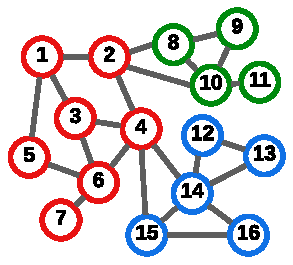
\includegraphics[width=0.18\linewidth]{out/about-frontier-01.pdf}
  }
  % \subfigure{
  %   \label{fig:frontier-example-02}
  %   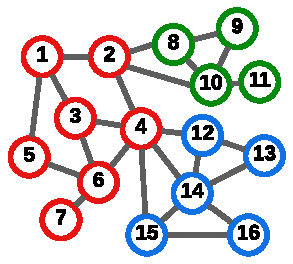
\includegraphics[width=0.15\linewidth]{out/about-frontier-02.pdf}
  % }
  \subfigure[]{
    \label{fig:frontier-example-03}
    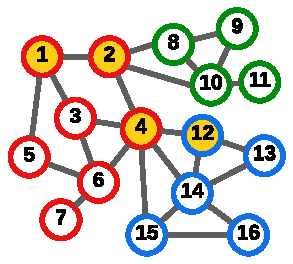
\includegraphics[width=0.18\linewidth]{out/about-frontier-03.pdf}
  }
  \subfigure[]{
    \label{fig:frontier-example-04}
    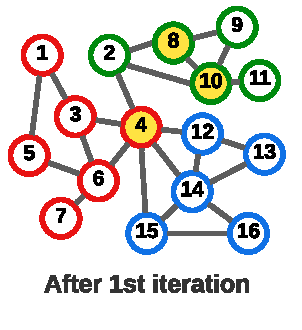
\includegraphics[width=0.18\linewidth]{out/about-frontier-04.pdf}
  }
  \subfigure[]{
    \label{fig:frontier-example-05}
    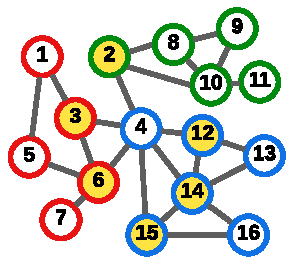
\includegraphics[width=0.18\linewidth]{out/about-frontier-05.pdf}
  }
  \subfigure[]{
    \label{fig:frontier-example-06}
    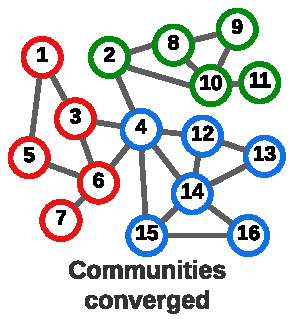
\includegraphics[width=0.18\linewidth]{out/about-frontier-06.pdf}
  } \\[-2ex]
  \caption{An example explaining the \textit{Dynamic Frontier} approach (\Fro{}). The community membership of each vertex is shown with border color (red, green, or blue), and the algorithm proceeds from left to right. A batch update arrives, affecting vertices $1$, $2$, $4$, and $12$. In the first iteration, vertex $2$ switches from red to green, impacting neighbors $8$ and $10$. In the second iteration, vertex $4$ changes from red to blue, affecting neighbors $3$, $6$, $12$, $14$, and $15$. Afterward, there are no more community changes.}
  \label{fig:frontier-example}
\end{figure*}
